\chapter{Experiments and Results}

In this chapter we will iterate through each of our initial objectives, analyzing their accomplishment and the obtained results.

\section{Objective 1. Maximize engagement of collaborators}

We will use our Personas from Section 4.1 to understand how would they use this tool and to check if their goals are met. The most difficult part of their job would be to get their hands on a client to collaborate on a problem they like. The top priority future work on this project would be building an online catalog where collaborators can easily look for problem they find interesting. Still let's assume our collaborators already have access to a client.

On the one hand, Aleix Vargas would probably use just the browser version of the client since he is not willing to install anything on his computer. He would only need to enter a valid URL on his browser and automatically start collaborating without having to mess around with download times, installation dependencies or execution parameters. 

The downside of browser client is that it might require to repeat these steps every time Aleix closes his browser and wants to start collaborating again. Nevertheless, as a work around, Aleix can pin the tab running the client or even setting it as his home-page so whenever the browser is started, the client is executed.

On the other hand, a collaborator more confident with their tech skills, like Ana Castillo, would rather use the native client in order to collaborate in projects they like. Installation however would require compilation for the architecture and operative system of the user. Fortunately, compiling Go code is really easy and precompiled binaries can be provided for different environments. Moreover, binaries for different combinations of operative systems and architectures can be compiled from the same machine by using command line instructions like on Listing \ref{lst:cross-compilation}.

\begin{lstlisting}[language=bash,
caption={Cross-compilation of client for different operative systems and architectures from the same Linux machine.},
label={lst:cross-compilation},
captionpos=b]
# Compile for Windows 64bits
GOOS=windows GOARCH=amd64 go build -o client.exe client.go

# Compile for Mac OS 64bits
GOOS=darwin GOARCH=amd64 go build -o client client.go

# Compile for Linux 32bits
GOOS=linux GOARCH=386 go build -o client client.go
\end{lstlisting} 

The main reason to use this kind of client is achieving higher performance than the browser-based client, and a less intrusive experience since the client can run in the background. Furthermore, the client can be scheduled to start running at log in so Ana do not need to start the client manually after she logs out on her computer.

An even more advance use case scenario would be a collaborator that wants to collaborate by creating a node and joining an already existing cluster as a new node to start collaborating on a problem they are interested in. The first step would be download the source code of a node for a given problem, building it, and running the executable, setting an already existing node in the cluster as bootstrapping node. In order to be able to receive migrations and requests from users, he will need to manually open ports on his router and forward incoming connection to his machine via port-forwarding.

All in all, for different types of user, given their tech skills and their objectives; this project provides solutions that do not differ much in terms of their implementations, and that cover their necessities.

\section{Objective 2. Fault-tolerant design capable of working with heterogeneous and ephemeral nodes}

As states in the previous section, Go is supported on many architectures and operative system. Implementation is usually architecture-agnostic which makes it a great language when one of the requirements of the final product is to support heterogeneous systems. Our implementation can be executed even on embedded systems which opens many opportunities with the currently increasing development of Internet of Things devices. A complete list of architectures and operative systems supported by Go can be found at \cite{go-architectures}.

Given the fact that we have built a collaborative system where we do not control the computation capabilities of the collaborating nodes, it is really important to be able to deal with a heterogeneous system where slower nodes can limit the performance of faster ones. This risk is minimized on our system using an asynchronous communications approach. 

On the one hand, clients evaluate individuals from the pool asynchronously thus a slower client cannot cause blocking on another client. On the other hand, migration is performed between islands from different nodes in a similar non-blocking approach where a separate thread from the main algorithm execution sends individuals to another node that handles the request on a separate thread from the main algorithm thread.

The only, but avoidable, temporal blocking situation of a client can happen due to a misconfiguration of the size of the population or the selection operator. If the population is too small, the time it takes to complete an iteration of the evolutionary algorithm over the individuals of an island can be superior to the time it takes to evaluate and return the modified individuals and therefore the next iteration of the algorithm will need to block until there are enough individuals in the population to apply the selection operator again. 

\begin{lstlisting}[
caption={Main loop of the evolutionary algorithm. If \textit{pool.NCandidates} (Line 6 and 9) equals to the size of the population, it can lead to a temporal blocking situation of the algorithm.},
label={lst:cross-compilation}, captionpos=b]
for pool.evaluations < pool.MaxEvaluations {
    var offsprings []eaopt.Individual

    // At least nOffsprings shold be available in the population
    // tu run this operator
    pool.popSemaphore.Acquire(pool.NCandidates)

    // take here randomly from population
    offsprings = pool.selection(4, pool.NCandidates)
    offsprings = pool.crossover(offsprings)
    offsprings = pool.mutate(offsprings)

    // Apply extra operators
    for i := range offsprings {
        for _, op := range pool.ExtraOperators {
            if pool.Rnd.Float64() <= op.Probability {
                offsprings[i].Genome = op.Operator(offsprings[i].Genome, pool.Rnd)
                offsprings[i].Evaluated = false
            }
        }
    }

    // Append non evaluated offspings to the channel and
    // Remove them from the population
    for i := range offsprings {
        if !offsprings[i].Evaluated {
            pool.population.Remove(offsprings[i])
            pool.evaluationChannel <- offsprings[i]
        } else {
            pool.popSemaphore.Release(1)
        }
    }
}
\end{lstlisting} 

On the other hand, even if the population is big enough to avoid the situation described above, if the selection operator is configured to perform a tournament with the same amount of individuals as in the population (i.e. the parameter $k$ of the selection operator equals to the size of the population), the algorithm will block until all clients return the evaluated individuals that have been modified in the previous iteration of the algorithm.

Fault-tolerance on a distributed system is another big challenge when working with ephemeral nodes that you do not control and are likely to stop working without previous notice nor troubleshooting options. Whereas by using a decentralized approach we achieve high reliability avoiding single point of failures on our system, there are other challenges to be addressed.

One the one hand, all nodes in the system must be able to reliably detect other faulty nodes to avoid expending time trying to communicate with them. This is achieved on Project\_Name by using a gossip protocol that detects node-failures and spread that information with low bandwidth usage and bounded time as it can be seen on Figure \ref{fig:failure_discovery_chart} and Table \ref{tab:failure_discovery_table}.

\begin{figure}[h!]
		\centering
    	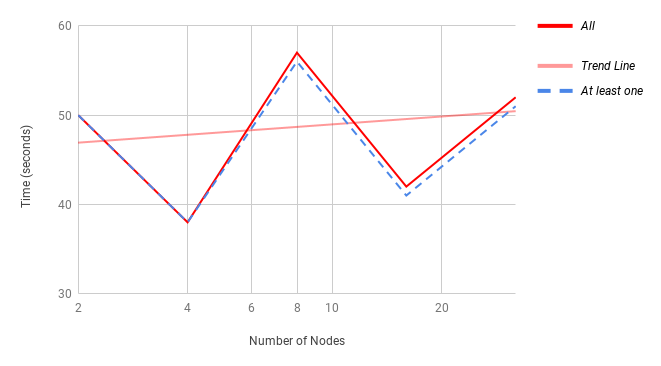
\includegraphics[width=\linewidth]{assets/images/Failure-detection-time.png}
    	\caption{\textbf{Failure detection times} depending on the number of nodes in the cluster. As it can be seen, time is bounded}
    	\label{fig:failure_discovery_chart}
\end{figure}

\begin{table}[h!]
\centering
\begin{tabular}{l|l|l|llll}
\cline{2-3}
                                     & \multicolumn{2}{c|}{\textbf{Time (seconds)}} &                       &                                       & \multicolumn{2}{c}{\textbf{}}                                                  \\ \cline{1-3} \cline{6-7} 
\multicolumn{1}{|l|}{\textbf{Nodes}} & \textbf{All}     & \textbf{At least one}     &                       & \multicolumn{1}{r|}{\textbf{}}        & \multicolumn{1}{l|}{\textbf{All}} & \multicolumn{1}{l|}{\textbf{At least one}} \\ \cline{1-3} \cline{5-7} 
\multicolumn{1}{|l|}{2}              & 50               & 50                        & \multicolumn{1}{l|}{} & \multicolumn{1}{r|}{\textbf{Average}} & \multicolumn{1}{l|}{47,8}         & \multicolumn{1}{l|}{47,2}                  \\ \cline{1-3} \cline{5-7} 
\multicolumn{1}{|l|}{4}              & 38               & 38                        & \multicolumn{1}{l|}{} & \multicolumn{1}{l|}{\textbf{Std}}     & \multicolumn{1}{l|}{7,69}         & \multicolumn{1}{l|}{7,46}                  \\ \cline{1-3} \cline{5-7} 
\multicolumn{1}{|l|}{8}              & 57               & 56                        &                       &                                       &                                   &                                            \\ \cline{1-3}
\multicolumn{1}{|l|}{16}             & 42               & 41                        &                       &                                       &                                   &                                            \\ \cline{1-3}
\multicolumn{1}{|l|}{32}             & 52               & 51                        &                       &                                       &                                   &                                            \\ \cline{1-3}
\end{tabular}
\caption{Raw data for failure detection times of Figure \ref{fig:failure_discovery_chart}.}
\label{tab:failure_discovery_table}
\end{table}

On the other hand, on a hypothetical scenario where nodes do not share the best solutions they find, if the node that has the best individual so far within the entire system fails, that solution will be lost and it is very unlikely to be recovered. By using the migration mechanism periodically and gossiping every individual that replaces the best one known so far on a node, our proposed design aims to avoid this scenario with eventual consistency.

To demonstrate this, we designed an experiment with a cluster of $N$ nodes where only one of them is having their individuals evaluated. We measured the time it takes for at least one other node, half of the nodes, 80\% of the nodes, and all the nodes, to receive a gossiped broadcast about an new best individual. The results, that can be found on Figure \ref{fig:broadcast_experiment} and Table \ref{tab:boadcast_experiment}, confirm that not only eventual consistency is met, but also most of the nodes receive the broadcast on a time that slowly increases with respect of the total number of nodes on the system. Note that even though it takes longer to broadcast an individual to all nodes, once most of them have received the broadcast, that information is unlikely to be lost.  Moreover, the time needed is likely to be smaller since on that experiment we deactivated migrations due to its selection method.

\begin{figure}[h!]
		\centering
    	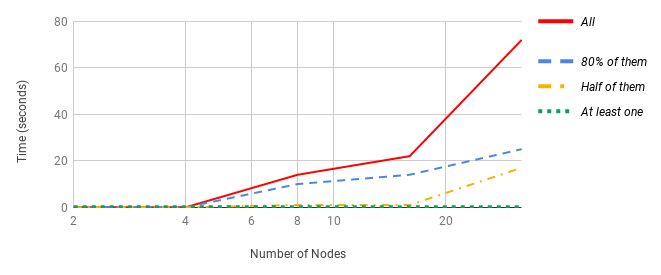
\includegraphics[width=\linewidth]{assets/images/broadcast-experiment.png}
    	\caption{\textbf{Broadcast times} depending on the number of nodes in the cluster. As it can be seen, Most of the nodes receive a broadcast on a time that slowly increases with respect of the total number of nodes.}
    	\label{fig:broadcast_experiment}
\end{figure}

\begin{table}[h!]
\centering
\begin{tabular}{l|l|l|l|l}
\cline{2-5}
                                     & \multicolumn{4}{c|}{\textbf{Time (seconds)}}                                                            \\ \hline
\multicolumn{1}{|l|}{\textbf{Nodes}} & \textbf{All} & \textbf{80\% of them} & \textbf{Half of them} & \multicolumn{1}{r|}{\textbf{At least one}} \\ \hline
\multicolumn{1}{|l|}{2}              & 0            & 0                    & 0                     & \multicolumn{1}{l|}{0}                    \\ \hline
\multicolumn{1}{|l|}{4}              & 0            & 0                    & 0                     & \multicolumn{1}{l|}{0}                    \\ \hline
\multicolumn{1}{|l|}{8}              & 15           & 10                   & 1                     & \multicolumn{1}{l|}{0}                    \\ \hline
\multicolumn{1}{|l|}{16}             & 22           & 14                   & 1                     & \multicolumn{1}{l|}{0}                    \\ \hline
\multicolumn{1}{|l|}{32}             & 72           & 25                   & 17                    & \multicolumn{1}{l|}{0}                    \\ \hline
\end{tabular}
\caption{Raw data for the broadcast times experiment of Figure \ref{fig:broadcast_experiment}.}
\label{tab:boadcast_experiment}
\end{table}

In conclusion, our system supports multiple operative systems and architectures, avoiding bottlenecks due to slower processors. Also, It provides a decentralized mechanism to achieve consistency and node failure detection that scales well with the number of nodes in the cluster.


\section{Objective 3. Achieve higher performance level than a non-distributed implementation}

In this section we will discuss the obtained results, comparing our distributed evolutionary model against a sequential implementation. There are two key aspects to analyze; throughput in terms of evaluations per second and solutions found after a given amount of time.

To analyze the throughput of our prototype, we have designed an experiment where we compare a sequential generational model against our distributed implementation. We will measure the average number of evaluated individuals per second for both models. We have deactivated the \textit{Train} operator for both scenarios since it can be a bottleneck for the maximum number of evaluations. In future releases it would be interesting to repeat this experiment enabling clients to perform other costly operators apart from the evaluation of individuals.

Figure \ref{fig:evaluations_experiment} shows the performance gain compared to a sequential generational model. As it can be seen, for just one (native) client, the sequential model slightly outperforms our implementation. This is expected since we have to pay a penalty in terms of latency on the communications between clients and islands.

However, form two clients on, our design is able to achieve a higher throughput than the generational model. Moreover, our design seems to scale pretty well with the number of clients, since as the number of clients increases, the throughput seems to increase almost linearly.

\begin{figure}[h!]
		\centering
    	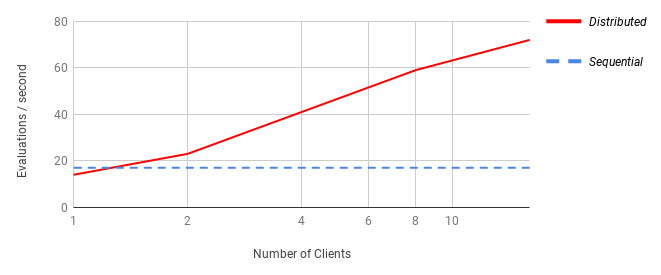
\includegraphics[width=\linewidth]{assets/images/experiment-evaluations-second.png}
    	\caption{\textbf{Evaluation performance.} The throughput in terms of evaluated individuals per second, seems to have linear performance gain with the number of clients.}
    	\label{fig:evaluations_experiment}
\end{figure}

\begin{table}[h!]
\centering
\begin{tabular}{|l|l|lll}
\cline{1-2}
\multicolumn{2}{|c|}{\textbf{Distributed model}}                          &           &                       & \textbf{}                                             \\ \cline{1-2}
\textbf{Clients} & \multicolumn{1}{c|}{\textbf{Throughput (Evals / Sec)}} &           &                       & \textbf{}                                             \\ \cline{1-2} \cline{5-5} 
1                & 14                                                     & \textbf{} & \multicolumn{1}{l|}{} & \multicolumn{1}{l|}{\textbf{Sequential model}}        \\ \cline{1-2} \cline{5-5} 
2                & 23                                                     &           & \multicolumn{1}{l|}{} & \multicolumn{1}{l|}{\textbf{Throughput (Evals /Sec)}} \\ \cline{1-2} \cline{5-5} 
4                & 41                                                     &           & \multicolumn{1}{l|}{} & \multicolumn{1}{l|}{17}                               \\ \cline{1-2} \cline{5-5} 
8                & 59                                                     &           &                       &                                                       \\ \cline{1-2}
16               & 72                                                     &           &                       &                                                       \\ \cline{1-2}
\end{tabular}
\caption{Raw data for the throughput experiment experiment of Figure \ref{fig:evaluations_experiment}.}
\label{tab:evaluations_experiment}
\end{table}

To analyze the capabilities of our prototype to find good solution, we have compared it against \textit{G-Prop} \cite{gprop} using the Glass problem described on previous sections. For this experiment, we set up 4 islands with 4 native clients each. A detailed list of the parameters of each algorithm can be found on Table \ref{tab:fitness-experiment-parameters}.

\begin{table}[h!]
\centering
\begin{tabular}{llll|l|l|}
\cline{1-2} \cline{5-6}
\multicolumn{2}{|c|}{\textbf{Gprop Parameters}}                              &  &  & \multicolumn{2}{c|}{\textbf{Godeea Parameters}} \\ \cline{1-2} \cline{5-6} 
\multicolumn{1}{|l|}{Population size}       & \multicolumn{1}{l|}{300}       &  &  & Island size                       & 100         \\ \cline{1-2} \cline{5-6} 
\multicolumn{1}{|l|}{Generations}           & \multicolumn{1}{l|}{500}       &  &  & Evaluations                       & 700         \\ \cline{1-2} \cline{5-6} 
\multicolumn{1}{|l|}{Selection rate}        & \multicolumn{1}{l|}{0.3}       &  &  & Cross Selection Tournament size   & 4           \\ \cline{1-2} \cline{5-6} 
\multicolumn{1}{|l|}{Mutation Prob}         & \multicolumn{1}{l|}{0.3}       &  &  & Mutation Prob                     & 0.3         \\ \cline{1-2} \cline{5-6} 
\multicolumn{1}{|l|}{Priority Mutate}       & \multicolumn{1}{l|}{1}         &  &  & Addition Prob                     & 0.3         \\ \cline{1-2} \cline{5-6} 
\multicolumn{1}{|l|}{Priority Addition}     & \multicolumn{1}{l|}{1}         &  &  & Elimination Prob                  & 0.15        \\ \cline{1-2} \cline{5-6} 
\multicolumn{1}{|l|}{Priority Elimination}  & \multicolumn{1}{l|}{1}         &  &  & Substitution prob                 & 0.15        \\ \cline{1-2} \cline{5-6} 
\multicolumn{1}{|l|}{Priority Training}     & \multicolumn{1}{l|}{1}         &  &  & Training Prob                     & 0.5         \\ \cline{1-2} \cline{5-6} 
\multicolumn{1}{|l|}{Initial wigths range}  & \multicolumn{1}{l|}{(0, 0.05]} &  &  & Migration size                    & 10          \\ \cline{1-2} \cline{5-6} 
\multicolumn{1}{|l|}{Weight mutation rate}  & \multicolumn{1}{l|}{0.005}     &  &  & Initial wigths range              & (0, 0.05]   \\ \cline{1-2} \cline{5-6} 
\multicolumn{1}{|l|}{LR mutation rate}      & \multicolumn{1}{l|}{0.005}     &  &  & Weight mutation rate              & 0,005       \\ \cline{1-2} \cline{5-6} 
\multicolumn{1}{|l|}{Hidden layer max size} & \multicolumn{1}{l|}{20}        &  &  & LR mutation rate                  & 0,005       \\ \cline{1-2} \cline{5-6} 
\multicolumn{1}{|l|}{Training Epochs}       & \multicolumn{1}{l|}{100}       &  &  & Hidden layer max size             & 20          \\ \cline{1-2} \cline{5-6} 
                                            &                                &  &  & Training Epochs                   & 100         \\ \cline{5-6} 
\end{tabular}
\caption{Parameters for the experiment. Parameters settings aim to be as close as possible between both algorithms. Population size and Generations for Gprop set for a execution time of about 60 seconds.}
\label{tab:fitness-experiment-parameters}
\end{table}

Table \ref{tab:fitness-experiment-results} shows the results of the experiment \footnote{The logs for this experiment can be found along with this document}. After about a minute of execution time, Godeea obtained better results than Gprop in terms of the number of failed predictions of samples from testing dataset (i.e. Prediction error).

Figure \ref{fig:fitness-experiment-evolution} shows the evolution of the fitness on the node that found the best solution at the end of the test. As can be seen, the average error, and the error of the best solution, decrease as the algorithm executes. Note that since the average fitness is printed every 100 evaluations, gaps have been filled with the previous value.

\begin{table}[h!]
\centering
\begin{tabular}{|l|l|l|l|l|}
\cline{1-2} \cline{4-5}
\multicolumn{2}{|c|}{\textbf{Gprop Results}} &           & \multicolumn{2}{c|}{\textbf{Godeea Results}} \\ \cline{1-2} \cline{4-5} 
Error                 & 73.58490566          &           & Error                 & 18.604651            \\ \cline{1-2} \cline{4-5} 
Time needed           & 61 seconds           & \textbf{} & Time needed           & 59 seconds           \\ \cline{1-2} \cline{4-5} 
\end{tabular}
\caption{Results of the experiment. As can be seen, Godeea obtains better results on the test dataset than Gprop.}
\label{tab:fitness-experiment-results}
\end{table}

\textbf{figure of how average fitness and best solution evolve on each node}.

\begin{figure}[h!]
		\centering
    	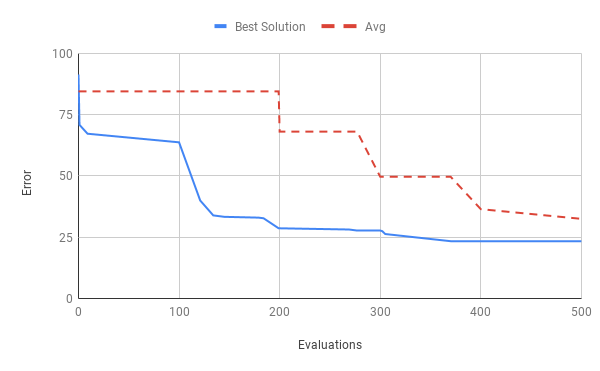
\includegraphics[width=\linewidth]{assets/images/experiment-fitness-evolution.png}
    	\caption{Evolution of fitness during the execution of Goodea on the experiment.}
    	\label{fig:fitness-experiment-evolution}
\end{figure}

\begin{table}[h!]
\centering
\begin{tabular}{|l|l|l|l|}
\hline
\multicolumn{1}{|c|}{\textbf{Evaluations}} & \multicolumn{1}{c|}{\textbf{Best Solution}} & \multicolumn{1}{c|}{\textbf{Avg}} & \multicolumn{1}{r|}{\textit{\textbf{Source}}} \\ \hline
0                                          & 91.43                                       & 84.51                             &                                               \\ \hline
1                                          & 70.87                                       & 84.51                             &                                               \\ \hline
9                                          & 67.25                                       & 84.51                             &                                               \\ \hline
100                                        & 63.74                                       & 84.51                             & \multicolumn{1}{r|}{\textit{broadcasted}}     \\ \hline
121                                        & 40.00                                       & 84.51                             &                                               \\ \hline
134                                        & 33.92                                       & 84.51                             &                                               \\ \hline
145                                        & 33.33                                       & 84.51                             &                                               \\ \hline
179                                        & 33.01                                       & 84.51                             &                                               \\ \hline
184                                        & 32.75                                       & 84.51                             &                                               \\ \hline
199                                        & 28.65                                       & 84.51                             &                                               \\ \hline
200                                        & 28.65                                       & 68.13                             &                                               \\ \hline
269                                        & 28.16                                       & 68.13                             & \multicolumn{1}{r|}{\textit{broadcasted}}     \\ \hline
277                                        & 27.74                                       & 68.13                             &                                               \\ \hline
300                                        & 27.74                                       & 49.68                             &                                               \\ \hline
302                                        & 27.49                                       & 49.68                             & \multicolumn{1}{r|}{\textit{broadcasted}}     \\ \hline
305                                        & 26.32                                       & 49.68                             &                                               \\ \hline
370                                        & 23.39                                       & 49.68                             & \multicolumn{1}{r|}{\textit{migration}}       \\ \hline
400                                        & 23.39                                       & 36.47                             &                                               \\ \hline
500                                        & 23.39                                       & 32.51                             &                                               \\ \hline
\end{tabular}
\caption{Raw data for Figure \ref{fig:fitness-experiment-evolution}. Blank \it{source} means that the best solution known so far was found on that node.  }
\label{tab:fitness-experiment-evolution}
\end{table}

All in all our design seems to outperforms sequential implementations in both throughput and final results, by scaling pretty well with the number of clients, and keeping a good balance between exploitation and exploration of the solutions search space as well.